\scanpage{18}
\mspage{7}
\margin{17}

Plus précisément, considérons le polygône combinatoire déduit du polygône combinatoire $\operatorname{Pol}(D)$ de $D$ sur $\operatorname{Str}(\underline\Sigma)$, en ``éclatant'' chaque sommet (correspondant à une arête de $\Gamma(\underline\Sigma)$ en $D$) en autant de sommets que l'indique son poids, et en plaçant sur chaque arête (correspondant à un coin de $\operatorname{Str}$ en $D$) autant de pts que l'indique son poids. On trouve un polygône $\widehat{\operatorname{Pol}}(D)$, \deleted{\unsure{Ceci dit,}} dont les sommets correspondent aux arêtes découpées sur \deleted{$\unsure{D}$} $\widetilde D$, visualisé comme un contour parallèle à $D$, \inserted{par les $\Delta_i$ ($\Sigma$);} (donc ses \uline{arêtes} correspondent aux sommets découpés par les $\Delta_i$ sur $\widetilde D$ --- \deleted{\unsure{de}} par $\Delta_i$ \deleted{\unsure{les éléments}} Si $I$ est l'ens d'indices pour $\Sigma$, $\widetilde I$ l'ens d'indices pour l'ens des $\vec\Delta_i$ orientés, on trouve donc une correspondance biunivoque can.
\[
\widetilde I\simeq\text{ens des arêtes de }\widehat P(D)
\]
d'où la relation \deleted{\unsure{de}} numérique plus haut. \deleted{\unsure{Cette}} Comme $\widehat P(D)$ est donc d'ordre $2n$, il admet une antipodie, $\widetilde I$ aussi --- et la bijection est compatible avec les antipodies.

\margin{\uline{NB} Le $\unsure{\widetilde{\widehat P}(D)|\widehat{\widehat P}(D)}$ défini \unsure{comme l'ens} des sommets de $\widehat P(D)$ qui étaient ``\unsure{au dessus}'' de sommets de $P(D)$, est stable pour l'antipodie.}

\deleted{\unsure{Ainsi} \illegible{2}} \unsure{À présent} examinons à part le cas de $D$ supercritique, soit \deleted{$\unsure{D}$}
\[
D\equiv\Delta=\Delta_{i_0},
\]
auquel cas il n'y a \deleted{\unsure{pas}} que des arêtes de généristé, issues de $D_j\to\Delta$, qui correspondent aux \deleted{\unsure{éléments}} \inserted{pts} de $\widetilde\Delta$ ($={}$ image inv. de $\Delta$ dans $\widetilde X$) qui sont au dessus des sommets sur $\Delta$.

\figure{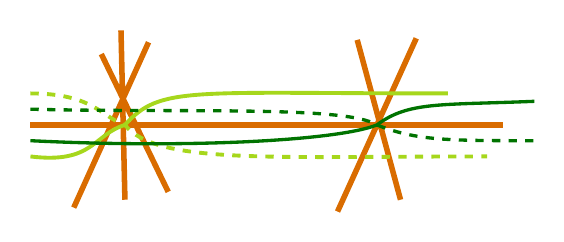
\begin{tikzpicture}[x=1cm,y=1cm]
\draw[orange!85!black,line width=2pt] (0,0)--(6,0);
\draw[orange!85!black,line width=2pt] (.55,-1.05)--(1.5,1.05) (1.2,-.95)--(1.15,1.2) (1.75,-.85)--(.9,.9);
\draw[orange!85!black,line width=2pt] (3.9,-1.1)--(4.9,1.1) (4.7,-.95)--(4.15,1.08);
\draw[yellow!65!green,line width=1.4pt] (0,-.4)..controls(.8,-.5)and(.8,-.12)..(1.2,0)..controls(1.65,.5)and(2,.4)..(5.3,.4);
\draw[yellow!65!green,line width=1.4pt,dashed] (0,.4)..controls(.8,.4)and(.9,.1)..(1.2,0)..controls(1.6,-.5)and(3,-.4)..(5.8,-.4);
\draw[green!45!black,line width=1.2pt] (0,-.2)..controls(2,-.3)and(3.9,-.2)..(4.4,0)..controls(4.8,.3)and(5.2,.25)..(6.4,.3);
\draw[green!45!black,line width=1.2pt,dashed] (0,.2)..controls(2,.15)and(4,.25)..(4.4,0)..controls(4.9,-.2)and(5.3,-.2)..(6.4,-.2);
\end{tikzpicture}}

\unsure{Choisissons} une orientation de $\Delta$, qui permet d'identifier $\widetilde\Delta$ en une des vis de $\Delta$. Nous affectons chaque arête \inserted{de $\Gamma(\underline\Sigma)$} issue de $\Delta$, \unsure{correspondante|correspondant} à \unsure{une généristé} $s\in S\cap\Delta$, des ``poids'' (\unsure{modifiés p.r.} à la définition précédente) égal au \deleted{\unsure{distinctes de $\Delta$},} \inserted{Nb.} des pdroites ($\Sigma_i$ \deleted{\unsure{qui sont}} \deleted{$\unsure{\Delta}$} \uline{distinctes de $\Delta$} qui passent en $s$, i.e. le nb de \uline{sommets} découpés au voisinage de $s$ par une ``parallèle'' (un côté) à $\Delta$.

\figure{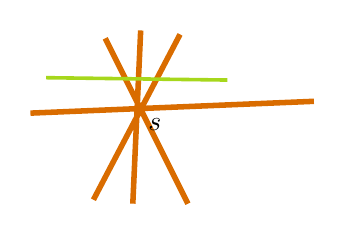
\begin{tikzpicture}[x=1cm,y=1cm]
\draw[orange!85!black,line width=2pt] (-1.4,0)--(2.2,.15) (-.6,-1.1)--(.5,1) (-.1,-1.15)--(0,1.05) (.6,-1.15)--(-.45,.95);
\draw[yellow!65!green,line width=1.3pt] (-1.2,.45)--(1.1,.42);
\node at (.18,-.15) {$s$};
\end{tikzpicture}}

Si nous ``éclatons'' chaque arête de $\Gamma(\underline\Sigma)$, en autant de sommets de
